\documentclass[11pt,letterpaper,twocolumn]{article}

% Provide an overview of the proposed research, including background, rationale,
% objectives and goals, research design, team, and feasibility. Describe how the
% project includes the appropriate and explicit incorporation of community
% engagement, Indigenous science and technology studies, or EDI as appropriate.
% Ensure that the significant project milestones and deliverables listed in the
% following milestones and deliverables section are clearly described and that
% you consider the ethical and sustainability of your project. Review the
% Application Guidelines to become familiar with evaluation criteria. (Maximum 3
% pages including key references, and supporting tables and figures).

% Essential packages
\usepackage[top=0.75in, bottom=0.75in, left=0.75in, right=0.75in]{geometry} % Tight margins
\usepackage{graphicx} % For figures
\usepackage{float} % Better figure placement control
\usepackage{caption} % For customizing captions
\usepackage{enumitem} % For compact lists
\usepackage{calc} % Required for \widthof command
\usepackage{titlesec} % For compact section headers
\usepackage{parskip} % No paragraph indentation, adds space between paragraphs
\usepackage{hyperref} % For clickable links and references
\usepackage{microtype} % Improves text appearance and spacing
\usepackage{csquotes}

\MakeOuterQuote{"}

% Compact section formatting
\titleformat{\section}{\normalfont\bfseries}{\thesection}{0.5em}{}
\titleformat{\subsection}{\normalfont\bfseries}{\thesubsection}{0.5em}{}
\titlespacing*{\section}{0pt}{1.5ex plus 0.5ex minus 0.2ex}{0.8ex plus 0.2ex}
\titlespacing*{\subsection}{0pt}{1.2ex plus 0.5ex minus 0.2ex}{0.6ex plus 0.2ex}

% Compact lists
\setlist{noitemsep, topsep=0pt, parsep=0pt, partopsep=0pt, leftmargin=*}

% Compact figure captions
\captionsetup{font=small, skip=4pt}

% Bibliography settings
\usepackage[numbers,sort&compress]{natbib}
\setlength{\bibsep}{0pt plus 0.3ex}

\title{\textbf{Team Chocolate: Optimizing Team Composition in Self-Driving Labs Through Bibliometric Analysis and Experimental Research}}
% \author{Sterling Baird et al.}
\date{}

\begin{document}

\maketitle
\thispagestyle{plain}

\section{Introduction}
Self-driving labs (SDLs) represent a new paradigm for materials discovery, combining automation, AI, and robotics to accelerate innovation\cite{sterling2024}. While technical aspects of SDLs are advancing rapidly, the optimal composition of research teams operating them remains understudied. Building interdisciplinary teams that integrate expertise in computer science, materials science, chemistry and engineering remains an unexplored challenge. This proposal investigates how team structure affects SDL research outcomes and productivity.

\section{Research Objectives}
We aim to answer three critical questions:
\begin{enumerate}
    \item How do team size and disciplinary diversity influence SDL research novelty and impact?
    \item What combination of specialists versus generalists maximizes SDL effectiveness?
    \item How do team dynamics and the mix of experience and expertise change with increasing levels of automation?
\end{enumerate}

Specifically, we will:
\begin{itemize}
    \item Assess how backgrounds and skill levels affect dimensions of performance
    \item Explore cross-disciplinary communication and troubleshooting strategies
    \item Document design choices in hardware, software, and AI implementations
\end{itemize}

\section{Methodology}
Our approach combines bibliometric analysis with experimental research and expert interviews:

\subsection{Research Team}
Our interdisciplinary team integrates expertise across economics, management, AI, materials science, and experimental design:
\begin{itemize}
    \item \textbf{Kristina McElheran, PhD (Lead PI):} Organizational economics and digitization expert who will coordinate the project and lead dissemination efforts
    \item \textbf{Marlene Koffi, PhD (Co-PI):} Early-career economist specializing in innovation and science with AI expertise; will lead bibliometric analysis and develop LLM-based tools
    \item \textbf{Megan MacGarvie, PhD:} Science of Science expert providing experimental design guidance through J-PAL networks
    \item \textbf{Aaron Clasky, PhD and Sterling Baird, PhD:} Materials science and SDL domain experts who will design experiments and provide insights on team dynamics
\end{itemize}

\subsection{Bibliometric Analysis}
We propose to collect bibliometric data from OpenAlex to comprehensively capture SDL-related publications, employing a dictionary-based method to identify these papers by developing a vocabulary of SDL-specific terms. This analysis will examine:

\begin{itemize}
    \item Author counts and disciplinary backgrounds
    \item Citation impact and degree of automation related to team structure
    \item Changes in team composition  across articles with differing degrees of automation, and over time as automation diffuses
    \end{itemize}
Additionally, curriculum vitae data from SDL authors will help analyze their career mobility and trajectories, assessing labor demand characteristics (e.g., academia versus industry) and the influence of SDL experience on their professional paths, and conducting gender disparity analyses inferred from profile images or names. 
% Example of efficient figure inclusion
\begin{figure}[H]
    \centering
    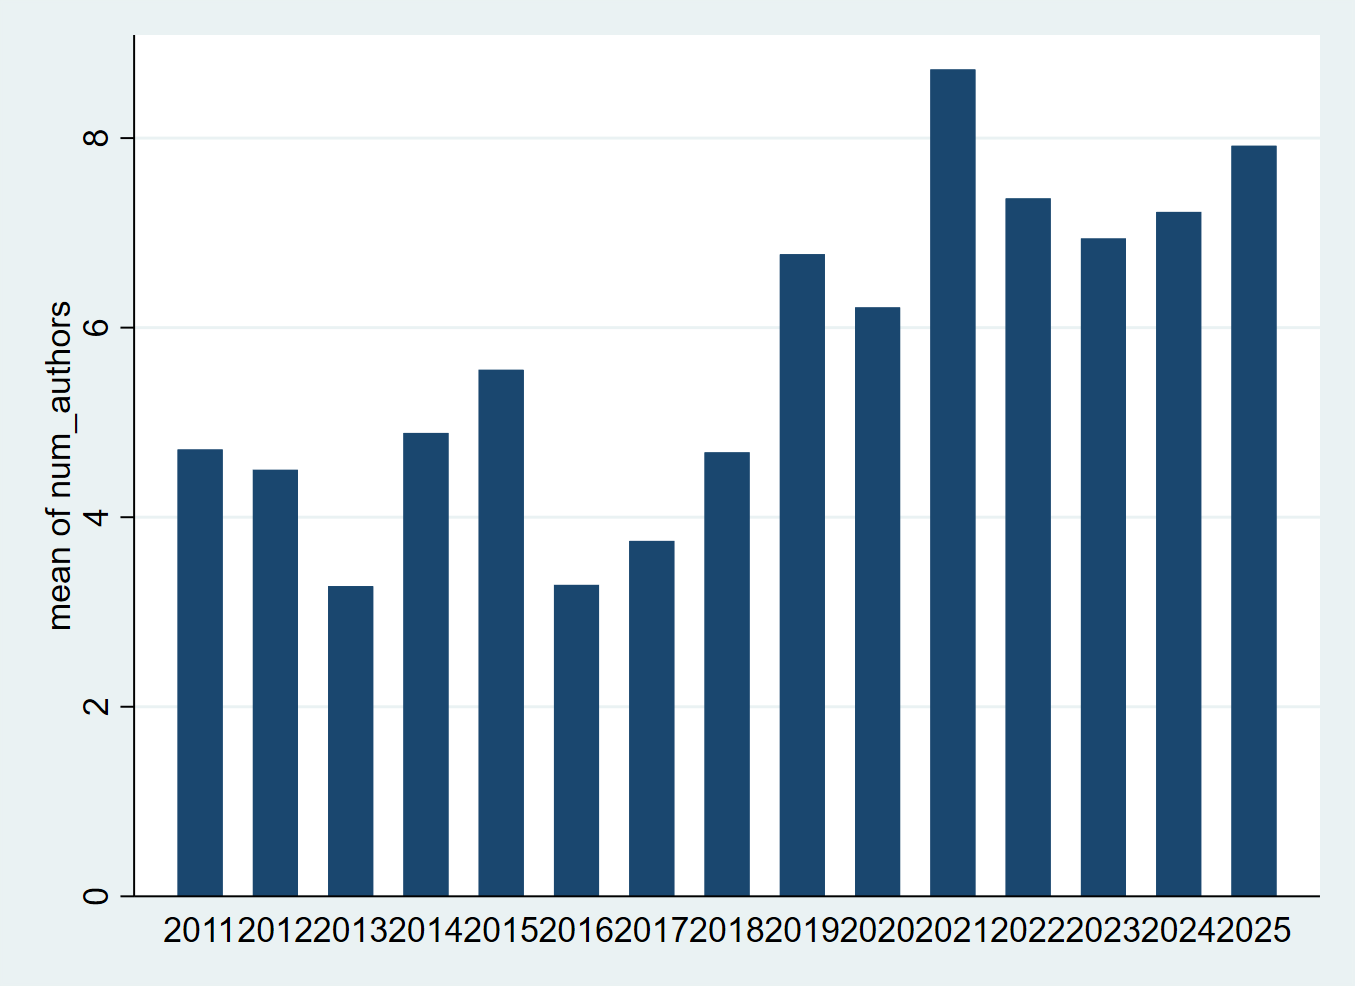
\includegraphics[width=0.9\linewidth]{num_authors.png}
    \caption{\small Average team size in SDL publications over time, demonstrating the evolving collaborative structure in this field.}
    \label{fig:team_size}
\end{figure}

\subsection{Experimental Study}
Building on insights from bibliometric analysis, we will conduct hackathon-style experiments using chocolate 3D printing as a model SDL system. Our "autonomous chocolatier" project leverages chocolate's phase-transition properties, which are analogous to metals, glass, and plastics, making it an ideal testbed for materials optimization. In this research:

\begin{itemize}
    \item Teams with varying compositions (e.g., different ratios of MSE, CS, and Mechanical Engineering students) will design autonomous chocolate formulation systems
    \item Specific team compositions will be determined based on findings from our bibliometric analysis
    \item Hardware integration will include chocolate 3D printers, powder and liquid dispensers, and robotic arms with a \$300 budget per team for additional equipment
    \item AI-driven decision tools will be integrated with hardware components to create a fully autonomous platform
    \item Materials will include 10 standard chocolate cores (620g) plus 2 non-standard cores per team
    \item Teams will be assessed on degree of automation, quality of final products, and system flexibility
\end{itemize}

\begin{figure}[t]
    \centering
    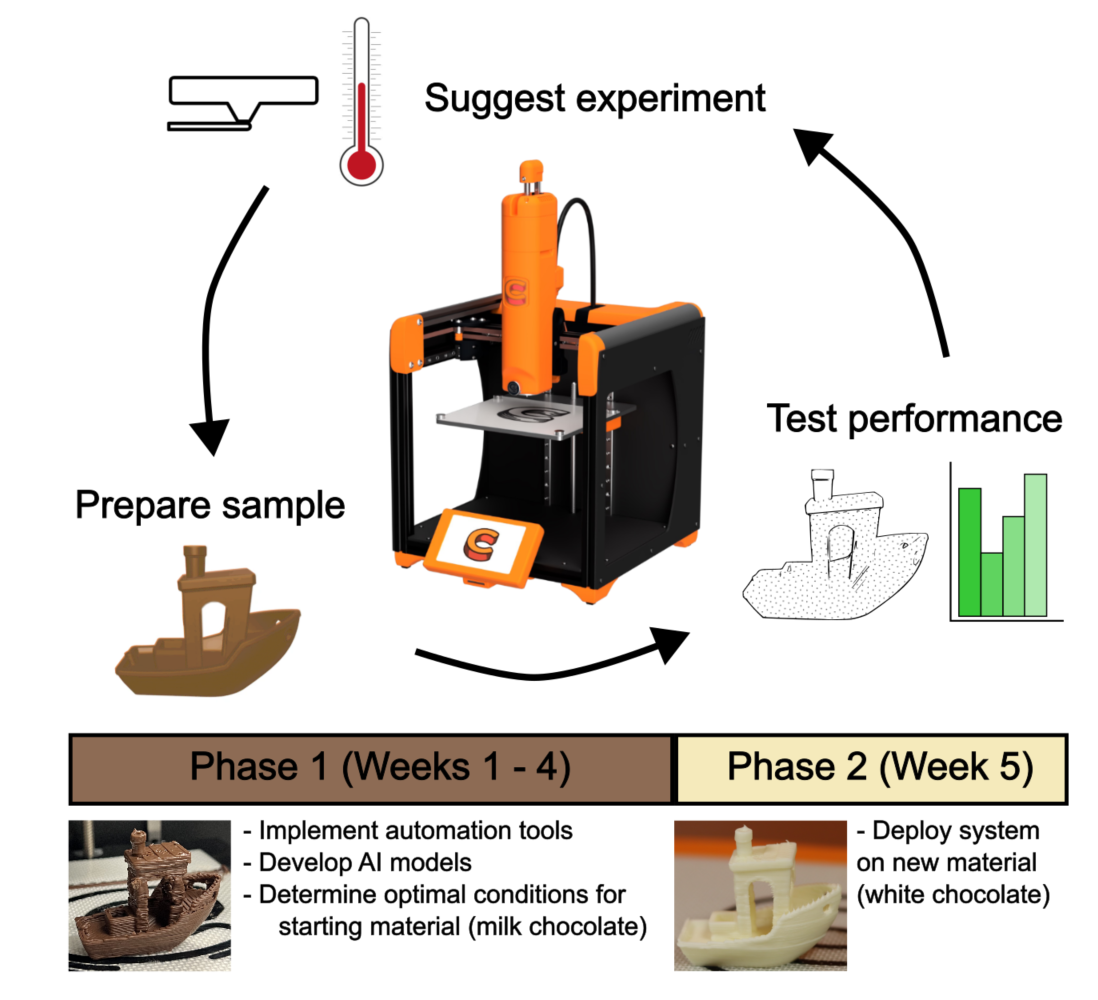
\includegraphics[width=0.49\textwidth]{chocolate-optimization-schematic.png}
    \caption{\small Schematic representation of our proposed chocolate optimization process as a model SDL system, illustrating how different team compositions will interact with the automated formulation platform. In the first four weeks, a team will create a system, testing it on milk chocolate. In the fifth week, teams will deploy their system on a new material (white chocolate), emulating industry-relevant settings where new formulations must be optimized as needs evolve.}
    \label{fig:chocolate_schematic}
\end{figure}

% Key research questions include:
% \begin{enumerate}
%     \item How does team diversity (specialist vs. generalist) affect the degree of automation achieved?
%     \item What team structures are most effective at building flexible systems that can adapt to new formulation challenges?
%     \item How do communication patterns differ between teams with varying compositions?
% \end{enumerate}

% \section{Anticipated Outcomes}
% This research will provide evidence-based guidance for:
% \begin{itemize}
%     \item Optimal SDL team structures across different research contexts
%     \item Training pathways for next-generation SDL researchers
%     \item Best practices for integrating domain expertise with automation capabilities
% \end{itemize}

\section{Timeline and Deliverables}
\begin{description}[leftmargin=!,labelwidth=\widthof{\bfseries 09/26-04/27:}]
    \item[05-09('25):] Data collection, experiment design, pilot studies
    \item[] Implementation of fully autonomous chocolate 3D printing platform, initial hackathon-style experiments
    \item[09-11('25):] Complete bibliometric analysis, finalize experimental protocols
    \item[12('25)-05('26):] Run experimental studies, collect and analyze data
    \item[06-08('26):] Complete integrated analysis of both research components
    \item[09('26)-04('27):] Prepare publications and practitioner guidelines
\end{description}

\section{Budget Summary}
Our budget of \$100,000 is allocated across three main categories:

\begin{itemize}
    \item \textbf{Personnel (\$52,349):} Three full-time undergraduate RAs for summer bibliometric data collection (\$34,595), plus one part-time RA continuing through academic year (\$16,108)
    
    \item \textbf{Equipment \& Materials (\$31,651):} Three sets of hardware including chocolate 3D printers and robotic arms (\$24,000), chocolate printing materials, sensors, documentation equipment, software licenses, and team budgets (\$7,651)
    
    \item \textbf{Dissemination (\$16,000):} Conference travel for team members (\$15,000) and production of best practices guide (\$1,000)
\end{itemize}

\section{Broader Impact}
This project will directly contribute to the Acceleration Consortium's mission by providing evidence-based strategies for structuring teams that maximize the potential of SDLs, ultimately accelerating materials discovery through optimal human-machine collaboration.

By analyzing team composition, dynamics, and outcomes in a controlled yet relevant setting, our research will offer actionable guidance for assembling effective SDL teams across academia, industry, and government. Our findings will inform best practices that can help scale the impact of SDLs and lower barriers to entry for new institutions seeking to establish their own automated materials discovery programs.

\section{Community Engagement \& EDI Considerations}
Our research design explicitly incorporates equity, diversity, and inclusion (EDI) principles in multiple dimensions:

\begin{itemize}
    \item \textbf{Inclusive Research Team:} Our team reflects a commitment to inclusivity, spanning gender and racial divides, with leadership from early-career and established researchers
    
    \item \textbf{Recruitment Practices:} RA recruitment will prioritize underrepresented backgrounds in STEM; hackathon-style experiments will emphasize diversity across gender, race, and discipline
    
    \item \textbf{Skills Development:} RAs will build both technical and collaborative research skills in a supportive, inclusive environment with intentional rotation of facilitation roles in team meetings to ensure equitable participation
    
    \item \textbf{Inclusive Technology Design:} Our experimental protocols will examine how team diversity affects the accessibility and inclusivity of resulting SDL systems
\end{itemize}

By embedding inclusion throughout the project, we aim to model how diversity strengthens scientific discovery while training the next generation of researchers.

\section{Ethical \& Sustainability Considerations}
We have carefully considered the ethical implications and sustainability of our research:

\begin{itemize}
    \item \textbf{Ethical Data Collection:} All bibliometric analysis and participant studies will follow IRB-approved protocols with proper consent and data anonymization
    \item \textbf{Environmental Sustainability:} Our chocolate-based experimental platform minimizes environmental impact by using biodegradable materials and energy-efficient processes
    \item \textbf{Long-term Impact:} By optimizing team structures for SDLs, we aim to accelerate sustainable materials discovery that addresses pressing global challenges
\end{itemize}

% Can include references as a list here rather than in-line to save space.
\bibliographystyle{unsrtnat}
\bibliography{bibliography}

\end{document}